\documentclass[11 pt]{article}
\usepackage[margin=1in]{geometry}
\usepackage{multirow}
\usepackage{multicol}
\usepackage{setspace}
\usepackage{epsfig}
\usepackage{times}
\usepackage{subfigure}
\usepackage{cite}
\usepackage{url}

\sloppy
\raggedbottom

\newcommand{\cellshade}[3]{\multicolumn{1}{>{\columncolor[gray]{#1}}#2}{\raisebox{-\belowrulesep}[0ex][8\aboverulesep]{#3}}}
\newcommand{\cellnoshade}[1]{\raisebox{-\belowrulesep}[0ex][8\aboverulesep]{#1}}
\newcommand{\mypar}[1]{\vspace{.0in}\noindent{\bf {#1}} \hspace{.04in}}
\newcommand{\myparnoskip}[1]{\noindent{\bfseries #1}\hspace{1em}}
\newcommand{\field}{\hspace{-.03in}\rightarrow\hspace{-.04in}}
\newcommand{\hd}{\sffamily\bfseries\footnotesize}
\newcommand{\hda}{\sffamily\bfseries}
\newcommand{\ie}{\emph{i.e.}, }
\newcommand{\eg}{\emph{e.g.}, }
\newcommand{\etc}{\emph{etc.}}
\newcommand{\etal}{, \emph{et al.}}

\newcommand{\myhline}{\begin{tabular}{l} \hspace*{3.0in} \\
      \hline\end{tabular}}
\newcommand{\myfullhline}{\begin{tabular}{l} \hspace*{6.4in} \\
      \hline\end{tabular}}
\newcommand\uclinux{{\aufnt $\mu$\emph{C}}{\tt linux} }

\newcommand{\ob}{}
\newcommand{\cb}{}

\def\sharedaffiliation{
\end{tabular}
\begin{tabular}{c}}


% For reducing item spacing in bulleted lists (see pg 166 of latex book)
\newcommand{\mybeginlist}{\begin{list}{\labelitemi}{\setlength{\itemindent}{0.0in}
\setlength{\topsep}{0.05in}\setlength{\partopsep}{0.0in}
\setlength{\itemsep}{0.0in}\setlength{\parsep}{0.0in}\setlength{\leftmargin}{0.17in}}}

\newcommand{\mybeginlistwithlabel}[1]{\begin{list}{#1}{\setlength{\itemindent}{0.0in}
\setlength{\topsep}{0.05in}\setlength{\partopsep}{0.0in}
\setlength{\itemsep}{0.0in}\setlength{\parsep}{0.0in}\setlength{\leftmargin}{0.17in}}}

\newcommand{\mybeginenumerate}{\begin{enumerate}{\setlength{\itemindent}{0.0in}
\setlength{\topsep}{0.05in}\setlength{\partopsep}{0.0in}
\setlength{\itemsep}{0.0in}\setlength{\parsep}{0.0in}\setlength{\leftmargin}{0.17in}}}


\begin{document}
\title{ \bfseries Retrofitting Security in COTS Software with Binary Rewriting}
%\author{P\'{a}draig O'Sullivan \and Rajeev Barua \and Angelos D. Keromytis}
% Authors taken out for blind review
\date{}
\maketitle

We present a practical tool for inserting security features against
low-level software attacks into third-party, proprietary or otherwise
binary-only software. We are motivated by the inability of software
users to select and use low-overhead protection schemes when source
code is unavailable to them, by the lack of information as to what (if
any) security mechanisms software producers have used in their
toolchains, and the high overhead and inaccuracy of solutions that
treat software as a black box.

Our approach is based on {\it SecondWrite}, an advanced binary
rewriter that operates without need for debugging information or other
assist. Using SecondWrite, we insert a variety of defenses into
program binaries. Although the defenses are generally well known, they
have not generally been used together because they are implemented by
different (non-integrated) tools. We are also the first to demonstrate
the use of such mechanisms in the absence of source code
availability. We experimentally evaluate the effectiveness and
performance impact of our approach. We show that it stops all variants
of low-level software attacks at a very low performance overhead,
without impacting original program functionality.


\section{Introduction}
\label{sec:introduction}

% Padraig: I just read the call for papers for ACSAC and it says the
% papers should be blinded.  Please read:
% http://www.acsac.org/2010/cfp/papers/ As a result, please remove the
% author names and all self-references.  Right now there are two I
% added: Matt's patent and kapil's pact paper.  Please replace those
% with new citations saying only "Suppressed for blind review."  You
% can leave the Secondwrite name there since no one yet knows where it
% comes from.  DONE

Despite considerable research and work on programmer education and
tools, programming language and compiler support for security,
hardware and operating system features, low-level software
vulnerabilities remain an important source of compromises and a
perennial threat to system security. While other sources of
vulnerability have emerged more recently, such as SQL injection,
cross-site scripting (XSS) and cross-site request forgery (XSRF),
binary-level vulnerabilities continue to be discovered in very popular
software \cite{flash-overflow,ms-overflows} and to be exploited for
fun and profit \cite{buffer-overflows}.

The lack of convergence to a comprehensive solution can be attributed
to several factors, consisting of a mix of the technical and
non-technical. At the core, there exists a fundamental dichotomy in
the capabilities and motivation of producers and consumers of
software, vendors and end-users/administrators respectively. On the
one hand, software producers are probably in the best position to both
proactively and reactively prevent and mitigate such vulnerabilities:
they have access to the source code, the compiler tool chain, and the
developers themselves. As a result, they can apply security mechanisms
that offer high coverage and effectiveness at low overhead, because
they are applied at the point where the most semantic knowledge about
the program and the code is available. On the other hand, it is
software consumers that face the risk and bear the costs of compromise
due to software vulnerabilities and are the most motivated to take
action, often localized, to mitigate a newly discovered
vulnerability. However, consumers often only have access to the
program binary and configuration files. Thus, absent vendor patches
(which can often take a long time and may contain bugs \cite{patches})
consumers can only use security mechanisms that treat the
software as a black box. Inevitably, such mechanisms resort to
isolation ({\it e.g.,} through a virtual machine) or to behavioral
detection ({\it e.g.,} system call monitoring), with attendant costs,
complexity and risk. Even security-conscious software consumers often
cannot properly evaluate the risks they face because they do not know
what security mechanisms, if any, a producer has used in their
development process and tool-chain \cite{securitybugs2003}.

% Padraig: Please fix all the XXX comments Angelos inserted above
% before returning the document to him for final review.  DONE -
% wasn't sure about the paper related to quality of patches but the
% paper I reference makes some compelling points that I thought made
% the same argument on the quality of patches. It also makes the point
% that patches for commercial products can take quite long to be
% released

We present a new mechanism based on advanced binary rewriting that
seeks to bridge the gap between incentive/motivation and capabilities
on the consumer side. Our approach allows end users to retrofit
powerful security mechanisms into third-party, binary-only
software. These mechanisms are well-known, and some of them have been
{\it partially} integrated in separate tools and development
environments ({\it e.g.,} ProPolice in {\it gcc} and the optional {\it
  /GS} flag in Visual Studio). Our system allows end-users to ensure
that the software they run on their systems uses any and all such
features, regardless of the choices or capabilities of
vendors\footnote{It is worth pointing out that not all development
  tool-chains support a given security feature, while vendors and
  products are often intimately tied to them. As a result, there is
  considerable reluctance by vendors to switch to a ``better''
  compiler, for example, even if such existed.}. Furthermore, our
approach allows end-users to selectively apply different defense
mechanisms to different parts of the program, based on their own
analysis, risk assessment, and knowledge of potential or actual
vulnerabilities in the code. Essentially, we provide the same
self-defense capabilities that open-source software users {\it can}
utilize to users of binary-only software\footnote{Of course, just
  because open-source software users {\it can}, does not mean they
  generally {\it do} assess or modify/secure their installations.}.

The contributions of this paper are twofold. First, we present a
powerful binary-rewriting framework in the context of software
security. Specifically, we investigate the ability of such a system to
retrofit known invasive, powerful and low-overhead security mechanisms
to program binaries, in the absence of source code or even debugging
symbols. Second, we evaluate the effectiveness and efficiency of our
scheme and of the retrofitted security mechanisms, as compared to
other ways in which these and similar security mechanisms can be
applied to software. We conclude that a system such as ours would
enable software consumers to protect themselves at the same level of
effectiveness as if vendors had taken similar steps ({\it i.e.,} used
the same security techniques) and at equally low overhead. Thus, we
believe that we have removed a significant factor in improving the
overall security posture of systems against low-level software
compromises.

An additional contribution of this paper is that we have carefully
chosen a set of complementary and effective schemes that, taken
together, achieve the goal of defending against all types of buffer
overflow attacks at the lowest combined run-time cost.  The totality
of our schemes protect against buffers on the global, stack, and heap
segments from overflowing onto a variety of (usually code) pointer
locations that are vulnerable to attack, including return
addresses, function pointers, indirect branch pointers, \emph{longjmp}
buffers, and base pointers. This is an important practical
contribution in itself, as this is the first solution in the
literature to retrofit a comprehensive set of protections against
buffer overflow attacks, which are still very common, into arbitrary
new and legacy binaries.  We intend to make this tool available
publicly soon.

The remainder of this paper is organized as
follows. Section~\ref{sec:related} gives an overview of related work
in binary rewriting and binary-only software security
mechanisms. Section~\ref{sec:background} presents background on binary
rewriting, and how rewriting relates to security. We describe the
methods we have chosen in Section \ref{sec:methods}, and discuss
experimental results in Section~\ref{sec:results}. We conclude with
our thoughts for future work in Section~\ref{sec:conclusions}.

\section{Related Work}
\label{sec:related}

Our work is related to many techniques that attempt to defend against
attacks on vulnerabilities in applications. In this section, we
elaborate on some of the pieces of work most closely related to
ours. We present the various attack techniques utilized by
attackers that are relevant for this research and then we go on to
present various techniques proposed for mitigating these attack
techniques. We also briefly discuss related work in
binary rewriting.

\subsection{Catalog of Attack Techniques}

\mypar{Buffer Overflow Attacks} A buffer overflow refers to a
situation that can occur when code writes into a bounded array, or
buffer, and the writes are not correctly guarded against
overflow. Data copied into the buffer whose length is larger than the
buffer's size is referred to as a buffer overflow. Writes into a
buffer that are not correctly guarded may overwrite and corrupt a
variety of vulnerable locations that may also be stored nearby the
buffer, including return addresses, base pointers, function pointers,
and \emph{longjmp} buffers. Although buffer overflows have
historically most often occurred on the stack, they are also possible
on heap and global segment buffers.  For example a global buffer's
overflow may overwrite a function pointer or \emph{longjmp} buffer
also in the global segment.

Buffer overflow attacks work by changing the value of the code pointer
stored in vulnerable locations such as return addresses, function
pointers and \emph{longjmp} buffers. The code pointer is overwritten
by a new value pointing to code of the attacker's choice.  Base
pointers are also vulnerable even though they are not code since they
can be used for attacks \cite{wilander2003}. A return address attack
was first described in detail by AlephOne in 1996
\cite{one1996}. However, attacks of this kind date back to before 1988
when the technique was used in the \begin{em}fingerd\end{em} exploit
  of the Morris worm.

Commonly, an attacker would choose their input data so that the
machine code for an attack payload would be present at the modified
return address. When the vulnerable function returns, and execution of
the attack payload begins, the attacker has gained control of the
behavior of the target software. The attack payload is often called
shellcode, since a common goal of an attacker is to launch a command
line interpreter (referred to as a shell in UNIX like environments)
under their control.

\mypar{Return-to-libc Attacks} As an alternative to supplying
executable code (referred to as direct code injection), an attacker
might be able to craft an attack that executes existing machine code
(indirect code injection). This class of attacks has been referred to
as jump-to-libc or return-to-libc (arc injection
\cite{cowan2000buffer} has also been used to refer to this class of
attacks) because the attack often involves directing execution towards
machine code in the standard C library (libc)
\cite{cowan2000buffer}. The standard C library is often the target for
attacks of this type since it is loaded in nearly every UNIX program
and it contains routines of the sort that are useful for an
attacker. This technique was first suggested by Solar Designer in 1997
\cite{designer1997return}. Attacks of this kind can evade defense
mechanisms that protect the stack such as stack canaries and it is
also effective against defenses that only allow memory to be writable
or executable.

Traditionally, attacks of this kind have targeted the system function
in the standard system library which allows the execution of an
arbitrary command with arguments. In this case, the return address of
a vulnerable function would be modified to point to the address of the
system function which would then be executed with attacker supplied
arguments. Since the system function executes a command on a system,
if an attacker can control the arguments to this function, they could
execute an arbitrary command on the system under attack. However,
recent attacks have been demonstrated which do not depend on calling
functions in the standard C library.

% Padraig: Please explain the exact mechanism of how the above
% return-to-libc attack works, for example the system function attack
% you mention above.  As this subsection is written now, I cannot
% understand how any return-to-libc attack works.  DONE

\subsection{Catalog of Defense Techniques}

\mypar{Compile Time Defenses} StackGuard \cite{stackguard-98} places a
'canary' (a memory location) on the stack between local variables and
the return address. This canary value is designed to warn of stack
corruption since validating the integrity of the canary value is an
effective means of ensuring that the function return address has not
been corrupted. Microsoft's compiler also supports the insertion of
stack canaries with the /GS option.

ProPolice \cite{eto2002propolice} is similar to StackGuard in that it
places a canary value on the stack. However, ProPolice also changes
the stack layout to place arrays and other function-local buffers
above all other function-local variables. Copies of all function
arguments are also made into new, function-local variables that also
sit below any buffers in the function. As a result, these variables
and arguments are not subject to corruption through an overflow of
these buffers.

PointGuard \cite{pointguard} protects all code pointers within a
program. The defense consists of encrypting pointer values in memory
and only decrypting the pointers when they are loaded into CPU
registers. The encryption key used is a randomly generated during
process creation and is thus unknown to an attacker. Without knowledge
of the encryption key, an attacker can not modify any value stored in
memory. As a result, pointer values are not subject to corruption.

StackGuard, PointGuard, and ProPolice involve compile-time analysis
and transformation. Thus, unless the source code for an application is
available, these techniques can not be used thereby hindering the
ability to easily deploy these techniques. In practice only the
developer can use these defenses, and only if the compiler his or her
organization uses supports it. Our techniques do not suffer from this
drawback since they can be easily deployed on any binary produced from
any source language and compiler, by not only the developer, but the
end-user as well.

% Padraig: the above paragraph references Pointguard, but it is not
% explained anywhere before that point.  Please fix.  DONE

\mypar{Instruction Set Randomization} Instruction-set randomization
\cite{isr} is a technique for protecting against buffer
overflows (and many kinds of code injection attacks). This approach
randomizes the underlying system's instructions so that foreign code
injected by an attacker would fail to execute correctly since the
attacker does not know the instruction set of the target
system. However, as mentioned by the authors in \cite{isr}, the main
drawback of this technique as applied to binary code that it needs
specialized hardware support in the processor. Thus, even though
instruction-set randomization offers a strong defense against buffer
overflow attacks the fact that unless it is supported by specialized
hardware, it incurs significant overheads means that it is unlikely to
see adoption in practice for the foreseeable future.

% Padraig: In dont understand the last two sentences.  If interpretive
% languages are not vulnerable, then how can the defense be effective?
% You can replace "are not vulnerable to" by "have not seen many".
% (or delete the two sentences) DONE - I removed the 2 sentences

Strata (a dynamic binary translation framework) and Diablo (a
link-time binary rewriter) were used to implement instruction set
randomization \cite{strata}. Diablo is used to prepare a binary for
string encryption and introduce the information necessary to detect
foreign code. Strata is then used to provide the necessary virtual
execution environment for safe execution. The main contribution of
this work is that the instruction-set randomization implementation is
efficient while requiring no special hardware support. However, the
runtime overheads reported are still high because of the necessary
software ISA translation at run-time, and the inherent overheads of a
dynamic translator. These run-time overheads and likely to limit the
practical adoption of such a system. Moreover any user of a dynamic binary rewriter must install it in addition to the application desired, making it inconvenient to use.

A static (off-line) binary rewriter such as the one used for our
research suffers from none of these issues. No special hardware is
required in order to utilize a binary rewriter and overheads are
relatively low since no ISA translation is done, and since no dynamic
translator is used, no additional software in addition to the application is needed for execution. In our system, if an original binary was compiled
without optimizations, we often see a significant run-time improvement
when rewritten.

\mypar{Address Space Layout Randomization} Address Space Layout
Randomization (ASLR) can be seen as a relatively coarse-grained form
of software diversity \cite{aslr}. ASLR shuffles, or randomizes, the
layout of software in the memory address space. The common
implementation of this scheme is at the OS level. Thus, when a process
is launched the address space layout of the process will be different
from a previous invocation of the same process. It is effective at
preventing remote attackers that have no existing means of running
code on a target system from crafting attacks that depend on
addresses. ASLR is not intended to defend against attackers that are
able to control the execution of a piece of software; it is mainly
intended to hamper remote attackers from attempting to use the same
attack repeatedly. Finally, its utility on 32-bit architectures is
limited by the number of bits available for address randomization
\cite{aslr32}.

% Padraig: (1) Who implements existing ASLR schemes -- a compiler,
% hardware, binary rewriter or OS?  Please clarify in above.  (2) Also
% you write "ASLR is not intended to defend against attackers that are
% able to control the software execution".  What does this mean?
% (Please rewrite to clarify.)  (3) I dont understand the scheme --
% does ASLR change the binary for each target system or once at
% compile-time?  If it is once then the randomized binary can be
% studied by the attacker and then attacked easily, is it not?  The
% basic problem is that the above paragraph does not clearly describe
% precisely what entity does ASLR or how it works and neither does it
% give an example of it.  Please rewrite to clarify all of these
% points.
%
% DONE - I attempted to address this. ASLR is not compile time, the
% address space is randomized each time a process is launched through
% a patch the loader in the operating system.


A binary rewriter could easily be used to provide a similar defense
mechanism as ASLR. An interesting future avenue of research is to
investigate software diversity through binary rewriting.

\mypar{Control Flow Integrity} Control Flow Integrity (CFI)
\cite{cfi-05} is a basic safety property that can prevent attacks from
arbitrarily controlling program behavior. CFI dictates that software
execution must follow a path of a control-flow graph that is
determined ahead of time by analysis (in this case, static binary
analysis is performed). CFI is enforced using static verification and
binary rewriting (with Microsoft's Vulcan \cite{vulcan} tool) that
instruments software with runtime checks. These checks aim to ensure
that control flow remains within a given control-flow-graph. CFI is a
very effective defense against buffer overflow attacks (and any attack
which attempts to change a program's control flow) since any attempt
by an attacker to divert the control flow of a program will be caught
by CFI. However, the main barrier to CFI's adoption seems to be the
overhead associated with the scheme. The average overhead of CFI in
the prototype implementation is 16\% on the SPEC2000 benchmarks. Also, unlike SecondWrite,
the binary rewriter used by CFI depends on a binary being compiled
with debug information which is usually not available in production
binaries. If a binary is not compiled with debug information then CFI
cannot be currently applied.

Our schemes implemented through our binary rewriter can provide the
same level of protection as CFI. An additional advantage of our scheme
is that our binary rewriter does not require access to any special
information in an input binary unlike all previous binary rewriters
(including the binary rewriter used in CFI) which require access to
relocation or debug information.

% Padraig: Please add a reference to the blank cite I added above for
% Microsoft's Vulcan tool.  DONE

\mypar{Program Shepherding} Program Shepherding \cite{shepherd}
employs an efficient dynamic software machine-code interpreter
(DynamoRIO \cite{drio}) for implementing a security enforcement
mechanism. A broad class of security policies can be implemented using
a machine interpreter such as DynamoRIO. For example, DynamoRIO could
be used to enforce control-flow integrity. Program shepherding
enforces a similar policy that imposes certain runtime restrictions on
control flow such that an attacker can not alter a program's flow of
control.

Program Shepherding can experience significant memory and runtime
overheads, particularly on the Windows platform. The scheme requires
an application and interpreter to be run simultaneously. The high
overheads of interpretation in some cases are likely to limit adoption
of Program Shepherding. Further, unlike using off-line rewriters like SecondWrite, Program Shepherding requires the installation of an extra piece of heavyweight software (DynamoRIO) in addition to the application to be run.

\subsection{Related Work in Binary Rewriting}

Binary rewriting and link time optimizers have been considered by a
number of researchers. Binary rewriting research is being carried out
in two directions: static rewriting and dynamic rewriting. Dynamic
binary rewriters rewrite the binary during its execution. Examples are
PIN \cite{pin}, BIRD \cite{bird}, DynInst \cite{dyninst}, DynamoRIO
\cite{drio} and Valgrind \cite{valg}. Dynamic rewriters are hobbled
since they do not have enough time to perform complex compiler
transformations; they have been primarily used for code
instrumentation and simple security checks in the past. Moreover
dynamic rewriters do not have the time to perform deep code analysis
needed to discover program features needed for static optimization of
security checks. Finally dynamic rewriters encounter run-time overhead
from the act of rewriting, which can be substantial. Given these
drawbacks, we do not discuss dynamic rewriters further.

The methods in this research are primarily directed at static binary
rewriters such as our rewriter, SecondWrite. Existing static binary
rewriters include Etch \cite{etch}, ATOM \cite{atom}, PLTO
\cite{plto}, Diablo \cite{Diablo1}, and Vulcan \cite{vulcan}. Three
points of novelty for our work are as follows. First, we are not aware
of any rewriter adding our particular set of existing compile-time
security schemes to binaries. Second, none of the existing rewriters
employ a compiler level intermediate representation; rather they
define their own low-level machine-code-like custom intermediate
representation. This has several downsides: $(i)$ most existing
rewriters cannot modify the stack layout since they do not distinguish
individual objects on the stack. Hence they cannot implement security
schemes that modify the stack; and $(ii)$ most existing rewriters
recognize functions, but not their arguments or return values, and
hence cannot deploy security schemes that employ these schemes. Our
Secondwrite rewriter overcomes both these problems; due to space
limitations, the pertinent details can be found elsewhere
\cite{blind-kapil}.

A third point of novelty of our work is that all existing rewriters
can only rewrite binaries that contain relocation or debug
information.  This information, present at link-time, is usually
discarded in COTS binaries for two reasons -- it is not needed for
execution; and vendors legitimately fear it can be used to reverse
engineer their binaries.  Indeed of twenty commercial and open-source
binaries we surveyed, \emph{none contained either relocation or debug
  information}.  As a result, existing binary rewriters would not be
able to rewrite those binaries at all.  \underline{In effect, existing
  binary rewriters can only be deployed by developers, not end-users.}
In contrast our rewriter (Secondwrite) can rewrite arbitrary binaries
even without relocation or debug information, as we have described in
previous work \cite{blind-matt}.  This renders our platform a uniquely
powerful tool for allowing anyone to rewrite binaries from any source
to enable any security scheme they want.

%Diablo defines an augmented whole program control-flow-graph based intermediate representation with program registers as globals and memory as a black box. It does not attempt to obtain high-level information like function prototypes and is geared mainly towards  optimizations like code compaction. Taking memory as a black box limits its applicability to architectures like x86 which have a limited set of registers. ATOM defines a symbolic RTL-based intermediate representation with infinite registers but does not make any attempt of analyzing or modifying the stack layout. Its mainly targeted towards RISC architectures. PLTO employs a whole program CFG based IR and implements stack analysis to determine the use-kill depths of each function. However, this information is not used for converting it into high-level IR; rather it is only used for low-level custom optimizations like load/store forwarding. Etch does not explicitly build an intermediate representation build an intermediate representation and allows users to add new tools to analyze binaries. The primary goal of Etch appears to be instrumentation and has only been shown to be applicable for simple optimizations like profile-guided code layout.
%
%
\subsection{Summary}

Current defenses have a number of weaknesses:

\begin{itemize}

\item They are not easily deployable

  \begin{itemize}
  \item Source code for an application is required
  \item An application needs to be compiled with certain information
  \item Hardware support is required
  \end{itemize}

\item Most are not readily available for use and evaluation

\item Some suffer from un-acceptable overheads

\item No scheme is immediately applicable to all binaries

\end{itemize}

Using the novel binary rewriting techniques developed within our research group, we have developed a scheme with the following characteristics:

\begin{itemize}

\item It is immediately deployable

\item It is applicable to any binary

\item Access to an application's source code is not required

\item An application does not need to be compiled in any way such that it contains special information e.g. debug or relocation information

\item It has low overheads

\item Many common stack-based buffer overflow attacks are prevented

\end{itemize}

%
% Padraig: I deleted the summary above and moved it to a file since I
% thought it was overly simplistic and unnecessary.  DONE - not really
% anything to do here...

\section{Background on binary rewriting}
\label{sec:background}

This section presents some background on binary rewriting and
discusses how security enforcement interacts with it. Our approach
relies on innovative binary rewriting
schemes~\cite{blind-kapil,blind-matt} incorporated into our binary
rewriting infrastructure called Secondwrite. Binary rewriters are
pieces of software that accept a binary executable program as input,
and produce an improved executable as output. The output executable
typically has the same functionality as the input, but is improved in
one or more metrics, such as run-time, energy use, memory use,
security or reliability.

\mypar{Advantages of binary rewriting} In recognition of its
potential, binary rewriting has seen much active research over the
last decade. The reason for great interest in this area is that binary
rewriting offers additional advantages over compiler-produced
optimized binaries:

\mybeginlist

\item \textbf{Ability to do inter-procedural optimization.} Although
  compilers in theory can do whole-program optimizations, the reality
  is that they do little if any. Many commercial compilers - even
  highly optimizing ones - limit themselves to separate compilation,
  where each file (and sometimes each function) is compiled in
  isolation. In contrast, binary rewriters have access to the complete
  application all at once, including libraries. This allows them to
  perform aggressive whole-program optimizations to exceed the
  performance of even optimized code. This ability can be useful for security schemes as well; in
    particular for those schemes that rely on whole-program information
    such as call graphs and inter-procedural properties to either work
    at all, or to optimize fully.

\item \textbf{Ability to do optimizations missed by the compiler.}
  Some binaries, especially legacy binaries or those compiled with
  inferior older compilers, often miss certain optimizations. Binary
  rewriters can perform these optimizations missed by the compiler
  while preserving the optimizations the compiler did 
  perform. This property may help the rewriter overcome some of the overheads
    of security enforcement by improvements in program run-time.

\item \textbf{Increased economic feasibility.} It is cheaper to
  implement a code transformation once for an instruction set in a
  binary rewriter, rather than repeatedly for each compiler for the
  instruction set. For example, the ARM instruction set has over 30
  compilers available for it, and the x86 has a similarly large number
  of compilers from different vendors and for different source
  languages. The high expense of repeated compiler implementation
  often cannot be supported by a small fraction of the demand. This
  implement-once property is useful for security schemes as well.

\item \textbf{Portable to any source language and any compiler.} A
  binary rewriter works for code produced from any source language by
  any compiler. This is a significant advantage when developing a
  security scheme such as the one presented in this paper. A scheme
  would not need to be ported to various compilers but would instead
  only need to be implemented once within a binary
  rewriter. Portability of rewriters aids security schemes implemented
  in them as well.

\item \textbf{Works for hand-coded assembly routines.} Code
  transformations cannot be applied by a compiler to hand-coded
  assembly routines, since they are never compiled. In contrast, a
  binary rewriter can transform such routines. Applying security in a
  binary rewriter has the advantage of working for hand-coded assembly
  versus compiler implementation of security, which does not.

\end{list}

%However, binary rewriters today have fallen far short of this desired
%vision. Binary rewriters remain relatively crude tools today, capable
%of no more than simple program transformations such as peephole
%optimization and code instrumentation. Complex transformations such
%as extensive whole-program optimizations, automatic parallelization
%and sophisticated security enforcement remain outside the
%capabilities of current rewriters.

% Padraig: I took the above paragraph out since the point here is to
% highlight all rewriters, not just ours.  Indeed it is not in the
% interests of this paper to make it seem like all the novelty is in
% our basic rewriter rather than your scheme.

\mypar{Architecture of Binary Rewriter} The binary rewriter developed
by our group and utilized for this research is named SecondWrite. Our
binary rewriter translates the input binary into the intermediate
representation (IR) of the LLVM compiler.  LLVM is a well-known
open-source compiler~\cite{llvm} developed at the University of
Illinois, and is now maintained by Apple Inc. LLVM IR is language- and
machine-independent. Our custom binary reader and de-compiler modules
read a binary and produce equivalent LLVM IR code.

Figure~\ref{swoverview} presents an overview of the SecondWrite
system. The SecondWrite system consists of a front-end module for
reading binary executables and generating an initial LLVM IR, an
internal pass module (not shown) for extracting more information about
the underlying program, optimizing passes to implement various
optimizations, and the LLVM code generator for producing the rewritten
binary.

\begin{figure}
\begin{center}
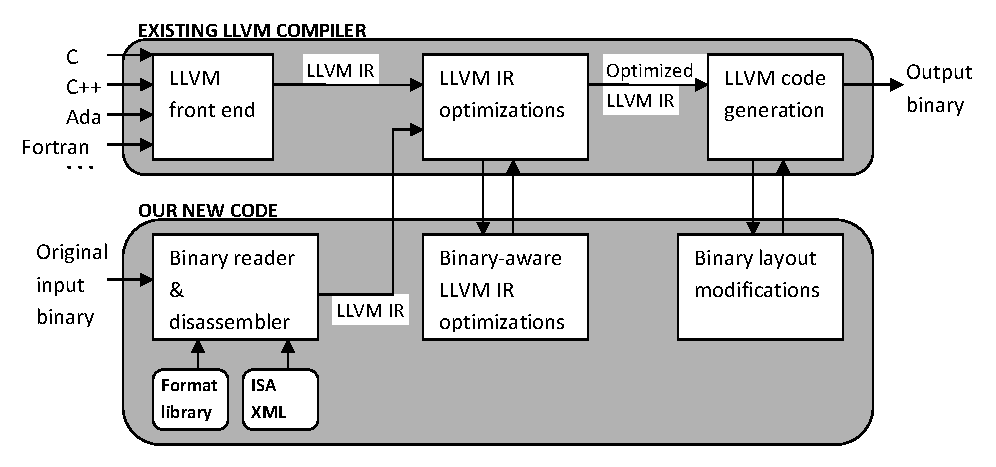
\includegraphics[scale=0.65]{images/flow.eps}
\end{center}
\renewcommand{\baselinestretch}{1}
\small\normalsize
\begin{quote}
\vspace{-0.2in}
\caption{SecondWrite system}
\label{swoverview}
\vspace{-0.5in}
\end{quote}
\end{figure}
\renewcommand{\baselinestretch}{2}

The front-end module consists of a disassembler and a custom binary
reader which processes the individual instructions and generates an
initial LLVM IR. This module reads the format of instructions from
Instruction Set Architecture (ISA) XML files for the ISA in question,
allowing for easy re-targeting of the rewriter to different
ISAs. Currently Secondwrite rewrites x86 and ARM binaries.

This initial representation is void of the desired IR features like
function prototypes, abstract stack and virtual registers. The
internal pass module analyzes this initial IR to obtain an improved IR
which has all the information and features mentioned
previously. Various existing and new LLVM optimization passes can be
applied on the above IR to obtain an optimized IR. Finally, the
optimized IR is passed to the existing LLVM code generator to obtain
the rewritten binary.

\mypar{Adding Security} Our approach to adding security to a binary is
to create numerous passes that work with the high-level IR. Working
with the high-level IR allows us to implement complex security
enhancements that would otherwise be difficult to add to a binary. We
discuss the various security methods we chose and implemented for this
paper in Section~\ref{sec:methods}. However, it is worth noting that
future research could easily focus on adding other security mechanisms
to the rewriter.


\section{Methods}
\label{sec:methods}

One of the contributions of this paper is that we have carefully
chosen a set of complementary and effective schemes that, taken
together, achieve the goal of defending against all types of buffer
overflow attacks at the lowest combined run-time cost.  The totality
of our schemes protect against not only the commonly known stack
buffer overflow into return addresses, but is much more general than
that, in that they protect against buffers on the global, stack and
heap segments from overflowing onto a variety of code pointer
locations that are possible in any data segment, including return
addresses, function pointers, indirect branch pointers, \emph{longjmp}
buffers, and base pointers\footnote{Base pointers are not code
  pointers but lead to a similar vulnerability \cite{wilander2003}.}.

We implement our scheme by adding various passes that operate on
high-level IR inside our binary rewriter. Our overall scheme consists
of a number of components that we describe in detail in this section.

\subsection{Stack Canary Insertion}

The first component of our scheme is the simplest. LLVM provides the
ability to insert stack canaries during code generation. Utilizing
this capability allows us to easily provide the same level
of protection to an un-protected binary as
StackGuard~\cite{stackguard-98} would provide when given an
application's source code.

Essentially, a random canary value is generated at run-time and placed
on the stack during a function's prologue. In the function epilogue,
the value stored on the stack is compared with the random canary value
for this process. If there is any difference, execution is halted as
the canary value has been corrupted.

\subsection{Base Pointer Elimination}

The \emph{old base pointer} which resides on the stack is a data
pointer that points to the base of the parent function's
stack frame. Compilers sometimes introduce it since it makes it
convenient to restore the stack pointer at the end of the function and
to address different stack locations with the same offset even as the
stack grows and shrinks in the function. When it is present in the
input binary, it introduces a vulnerability just as dangerous as a
code pointer~\cite{wilander2003}. This is because the old base pointer
can be attacked by building a fake stack frame with a return address
pointing to attack code, followed by overflowing the buffer to
overwrite the old base pointer with the address of this fake stack
frame. Upon return, control will be passed to the fake stack frame
which immediately returns again redirecting flow of control to the
attack code.

Given our unique use of LLVM IR in Secondwrite, the elimination of the
base pointer in the output binary becomes a simple matter even when
the input binary has base pointers. LLVM is an optimizing compiler and
the binaries produced by LLVM are highly optimized. One common
optimization applied by modern compilers on the x86 platform is to
free up the EBP register for register allocation by removing the base
(or frame) pointer. We used this LLVM pass to eliminate the base
pointer from the binary.

When the base pointer is eliminated by LLVM, any attack relying on overwriting the base pointer
is immediately prevented. There will be no base pointer for an
attacker to modify. While corruption of the stack may still occur if
an attacker overflows a buffer in order to attempt to overwrite the
base pointer, no attack will be successful.

\subsection{Return Address Protection}

Given that stack canaries as inserted by LLVM do not provide the same
level of protection as the ProPolice mechanism that comes with GCC, we
decided to implement a more complete solution similar to the
protection scheme in StackShield \cite{stackshield}, that protects
against corruption of the return address. The basic idea of our return
address protection scheme is as follows:

\mybeginenumerate

 \item During the function prologue, push the return address of the
   current function in a return address stack implemented in a global
   variable.

 \item In function epilogue, compare the current return address on the
   stack with the value popped from the top of the return address
   stack.

 \item If there is any difference between these values, execution is
   halted.

\end{enumerate}

This simple scheme will detect if the return address has been modified
either directly or indirectly. We implemented this scheme as it is
relatively simple and protects against both direct and in-direct
modifications of the return address. It also requires no modification
of the stack layout and prevents modifications of the return address
through buffer overflows in the heap or global segments.

Two challenges with this scheme are as follows. First, its overhead
might be significant since every function has an associated security
overhead incurred every time it is called. We found this overhead to
be especially significant for recursive functions since they tend to
short-running. Second, the size of the return address stack might be
significant for deeply nested recursive functions, and we would have
to bound it a-priori, which is hard to do.

We applied an optimization for relieving this problem which we call
the \emph{return address check optimization}. We observed that this
protection mechanism is only necessary if a function contains a write
to a stack buffer since return addresses only exist on the stack. This
is hard to determine without symbolic information, so we
conservatively try to prove that a function only has directly
addressed memory references to constant addresses.  If it finds any
indexed write (base + runtime-variant offset), then it conservatively
assumes that it could be a buffer write, and disables the
optimization. If all writes are provably non-indexed writes to a
constant offset, it enables the optimization, \ie the protection
mechanism is turned off in the function. Thus the optimization saves
on run-time overhead without sacrificing any protection.

% Padraig: Please complete the above paragraph.  Talk about why you
% think this scheme is better than stack canaries and propolice.  DONE

% Padraig: In the results section we should present results on the
% impact of the return address check optimization.  NOT DONE - raw
% numbers have been collected but not sure how to show this and stay
% within the page limit required for the conference

We found this optimization surprisingly effective since it works best
for small leaf functions in the call graph, and for recursive
functions, which happen to be precisely the functions dynamically
called most frequently.  During our experimental evaluation of our
scheme, of the many recursive functions we found, every one of them
had its check optimized away.  This is unsurprising since recursive
functions tend to be short running, and unlikely to allocate stack
arrays (although they may access portions of global arrays, such as in
quicksort, but those still are optimized.)  As a result of the
optimization, the run-time overhead for scheme is greatly reduced, and
the required return address stack depth is also greatly reduced.  Of
course, the overflow of the return address stack is not an error as we
add extensions to it on the heap upon overflow, which slows execution,
but is extremely rarely invoked even for small return address stack
sizes of (say) 256 addresses.

\subsection{Function Pointer Protection}

One common attack method used by attackers is to overwrite a function
pointer so that when it is de-referenced, code of the attacker's
choosing will be executed. In a binary executable, function pointers
will appear as indirect calls. Thus, another component of our scheme
concentrates on protecting all indirect calls and branches similar to
how function pointers are protected in StackShield \cite{stackshield}.

Our scheme adds checking code before all indirect calls and
branches. A global variable is declared at the end of the data segment
and its address is used as a boundary value. The checks inserted
before any indirect call or branch ensure that the target of the
indirect call or branch points to memory below the address of the
global boundary variable. If the target points above the address of
this global boundary variable then execution is halted.

% Padraig: Need to explain why the above scheme works.  What invariant
% are you assuming about the way OSs lay out the global and code data
% segments?  You should allow the function pointer to point to the
% code segment, but not the data segments, and not dlls either.  How
% does the above scheme ensure that? Does the scheme work when the
% attacker changes the function pointer to point to the C library
% (return-to-libc attack?)  DONE

An assumption in the above scheme is that a process follows the
standard UNIX layout with the data segment above the code
segment. This scheme does not protect against return-to-libc attacks
since the target of the indirect call will still be within the code
segment.

\subsection{Protection for \emph{longjmp} buffers}

The paired functions \emph{setjmp} and \emph{longjmp}, present in most
C and C++ libraries, provide a means to alter a program's control flow
in addition to the usual subroutine call and return sequence. First,
\emph{setjmp} saves the environment of the calling function (say
\emph{foo()})into a data structure, and then \emph{longjmp} in another
function (say \emph{bar()}) can use this structure to jump back to the
point it was created, at the \emph{setjmp} call. As a result,
execution will return from \emph{bar()} to \emph{foo()} even when
\emph{foo()} is not the immediate parent of \emph{bar()}. A typical
use for \emph{setjmp}/\emph{longjmp} is exception handling.

The data structure used by \emph{setjmp} for saving the execution
state is referred to as a \emph{jmp\_buf}. Within this structure,
enough information is stored to restore a calling environment. In
particular, one member of this structure saves the value of the
program counter which is used when restoring the calling
environment. An attack method used by attackers is to overwrite the
value of the program counter stored in the \emph{jmp\_buf} structure
after a call to \emph{setjmp} and before a call to \emph{longjmp}. If
this happens, control will be transferred to an address of the
attacker's choosing when the \emph{longjmp} is executed. Our method
for defending against attacks of this kind is as follows:

\mybeginenumerate

 \item Create a hash table within the global segment of the rewritten
   binary.
 \item After each call to \emph{setjmp} store the current value of the
   program counter member of the \emph{jmp\_buf} structure in the hash
   table.
 \item Before a call to \emph{longjmp} get the current value of the
   \emph{jmp\_buf} structure that will be used. Attempt to perform a
   lookup in the hash table for the value of the program counter.
 \item If the lookup in the hash table fails, then the value of the
   program counter has been modified and so we abort; otherwise
   execution continues

\end{enumerate}

We expect the run-time overhead of this scheme to be very low in
practice, since \emph{setjmp} and \emph{longjmp} calls are very
rare. To the best of our knowledge, this scheme is the first
protection scheme designed to protect against longjmp buffer attacks
in the manner described.

% Padraig: You need to say here if this method is a new method of our
% creation, an existing method, or a variant of an existing method.
% In the later two cases, give a reference.  If it is new, say so and
% claim credit for it!  DONE

\section{Experimental Evaluation}
\label{sec:results}

We now present and discuss experimental results from our evaluation of
our system. First, we examine the effectiveness of our security
schemes as implemented in SecondWrite on a set of security benchmarks
previously proposed by Wilander and Kamkar~\cite{wilander2003} for
evaluating the effectiveness of buffer overflow defenses. Second, we
examine how effective our scheme is in protecting against real-world
attacks on widely-used real code (not benchmarks). Third, we examine
the overheads of both the binary rewriter and our security scheme on
some SPEC2006 and other benchmarks.

\mypar{Synthetic Results} In order to test how effective our scheme
is, we utilized the benchmarks provided by Wilander and Kamkar
\cite{wilander2003}. Twenty buffer overflow attack forms were
developed, in order to evaluate the effectiveness of tools available
at the time that aimed to mitigate buffer overflow attacks. The attack
forms covered every combination of buffer overflow attacks on global,
stack, and heap buffers overflowing to a return addresses, base
pointers, function pointers, and \emph{longjmp} buffers. An attack
form is defined as a combination of a technique, location, and an
attack target. Of the twenty attack forms, we obtained the source code
to only eighteen of these attack forms. We then compiled the programs into binary code which we then rewrote using SecondWrite.
Our schemes in SecondWrite successfully
defended against all attack forms in the Wilander and Kamkar
benchmarks.

\mypar{Real World Attacks} Ultimately, the success of our scheme depends on whether or not attacks that are observed in the real world can be prevented or not. Two real-world attacks were tested.

The first application we tested was a HTTP server named GHTTPD. This web server has a stack buffer overflow vulnerability in its logging function \cite{ghttpd}. We obtained an exploit for this application which overflows a stack-based buffer and corrupts the return address. Using the return address protection component of our scheme, we were able to protect the return address and prevent the attack that uses the buffer overflow vulnerability to  corrupt the return address. When our protection scheme is enabled, the return address corruption is detected when the attack occurs and the application is aborted.

% Padraig: Give a reference to the GHTTPD attack.  Even a website reference is fine.
% DONE

The second application we tested was another HTTP server named CoreHTTP. This application contains a buffer-overflow vulnerability where it fails to adequately check user-supplied data before copying it to an insufficiently sized buffer \cite{corehttp}. We obtained an exploit for this application and applied our protection scheme to the application. Again, when our protection scheme is enabled, the attack is detected and the application is aborted.

\mypar{Binary Rewriting Overhead} A subset of SPEC benchmarks and
other benchmarks were selected to substantiate the performance of our
binary rewriter. The benchmarks were selected at random, and
are limited only by the criteria that they are correctly rewritten by
our still-early prototype. Table~\ref{benchlist} lists the set of
benchmarks that are used in the experiments. All the benchmarks are
compiled with gcc 4.4.1.

% Padraig: This section in two places (here and at the beginning of
% the section talks about "SPEC and other" benchmarks.  It is possible
% that by Friday when Kapil submits his paper all his benchmarks will
% be SPEC, in which case you can use those and take out the "and
% other" phrase.

\begin{table}
\begin{center}
\begin{tabular}{ | c | c | c | }
\hline
\textbf{Application} & \textbf{Source} & \textbf{Lines of C Source Code} \\
\hline
\hline
lbm & SpecFP2006 & 1155 \\
\hline
art & OMP2001 & 1914 \\
\hline
mcf & SpecInt2006 & 2685 \\
\hline
libquantum & SpecInt2006 & 4357 \\
\hline
sjeng & SpecInt2006 & 13847 \\
\hline
hmmer & SpecInt2006 & 35992 \\
\hline
h264 & SpecInt2006 & 51578 \\
\hline
\end{tabular}
\end{center}

\caption{Application Characteristics}
\label{benchlist}
\end{table}

In the first experiment, all binaries executed correctly after
rewriting thereby demonstrating the robustness of our binary
rewriter. We were able to correctly apply the standard suite of LLVM
optimization passes without any changes. These include CFG
simplification, global optimization, global dead-code elimination,
inter-procedural constant propagation, instruction combining,
condition propagation, tail-call elimination, induction variable
simplification and selective loop unrolling.

Besides correctness, the next most important metrics are the run-time
speedup or overhead of the rewritten binaries versus the input
binaries. For this paper, we study the performance of our rewriter on
already optimized binaries. Figure \ref{withopts} shows the normalized
execution time of each rewritten binary compared to an input binary
produced using GCC with the highest available level of optimization
(-O3 flag). The results are mixed, with most benchmarks
nearly breaking even or showing a small slowdown, one benchmark
showing a larger slowdown of 20\%, and one benchmark actually shows a
speedup of 16\%. The average is 3\% slowdown.\footnote{Rewriting unoptimized input binaries produced using GCC -O0 yields an average speedup of 27\% using SecondWrite (not shown) due to its optimizations.}

\begin{figure}[ht!]
\begin{center}
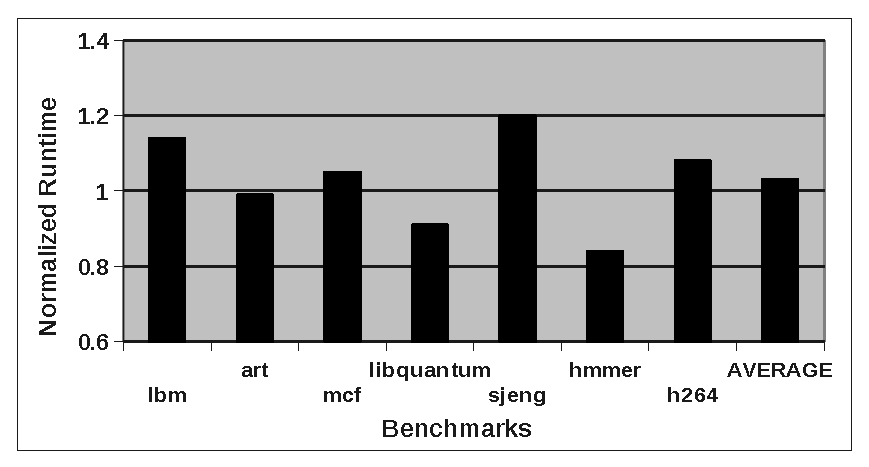
\epsfig{file=images/perfopt4.eps}
\par\end{center}
%\renewcommand{\baselinestretch}{1}
%\small\normalsize
%\begin{quote}
\vspace{-.2in}
\caption{Normalized runtime of rewritten binary as compared to optimized input
  binary (runtime=1.0).}
\label{withopts}
%\end{quote}
\end{figure}
%renewcommand{\baselinestretch}{2}

We consider this near break-even performance on highly optimized
binaries a good result for the following three reasons:

\mybeginlist

\item Our initial goal was not necessarily to get a speedup, but to
  generate correct IR without without introducing too much
  overhead. This would enable the IR to be a starting point for
  various custom compiler transformations we wanted to perform
  thereafter, such as automatic parallelization or security as covered
  in this thesis. Ultimately, these optimizations determine the
  utility of the rewriter.

\item These numbers represent our first-cut implementation devoid of
  any attempt at producing a better IR more geared towards
  optimization. We believe these numbers can be substantially improved
  with more detailed IR and are exploring several related avenues.

\item We have currently not implemented any custom serial
  optimizations that might improve performance further, such as the
  inter-procedural versions of common sub-expression elimination and
  loop-invariant code motion, changing the compiler-enforced calling
  convention for registers for better run-time, and more aggressive
  inlining. We believe these optimizations hold promise as the
  inter-procedural optimization abilities of current compilers are
  very limited compared to their intra-procedural performance.

\end{list}

One additional advantage of the binary rewriter is that it accumulates
optimizations across two compilers---rewritten binaries have an
optimization if it is either present in the compiler that produced the
input binary, or in the rewriter. In our case, if either GCC or LLVM
had an optimization, the output binary should have it. This is why,
for example, one of our rewritten binaries (\emph{hmmer}) had a 16\%
speedup versus the input binary. Although GCC with the -O3
optimization flag is known to produce good code, in some cases it
missed promoting structure fields to registers whereas LLVM did,
explaining the speedup in \emph{hmmer}. With better IR and more
aggressive optimizations, we expect to see more consistent speedups in
output binaries in the future.

\mypar{Security Related Overheads} The overhead of the security
schemes was measured on the same applications as used for
measuring the overhead of the binary rewriter. The results are presented in Figure \ref{fig:security} and show overhead versus rewritten binaries without security schemes inserted. As seen, the average run-time overhead of 7\% introduced by the protection scheme is low.

\begin{figure}[ht!]
\begin{center}
\epsfig{file=images/sec.eps}
\end{center}
%%\renewcommand{\baselinestretch}{1}
%%\small\normalsize
%%\begin{quote}
\vspace{-.2in}
\caption{Normalized runtime of rewritten binary with security scheme added.}
\label{fig:security}
%%\end{quote}
\end{figure}
%%\renewcommand{\baselinestretch}{2}

%Next, we measured the overheads of adding the protection scheme to the applications we used for our real-world experiments. These results are presented in Figure .

\section{Conclusions}
\label{sec:conclusions}

We have presented a new mechanism using an advanced binary rewriter
that allows end users to retrofit powerful security features into
third-party, binary-only software. The particular mechanisms we used
are well known, and some have been partially implemented in other
tools.  Our system will allow end-users to retrofit program-level
security protections for the first time in a highly customizable
manner according to their needs and environment.

We demonstrated the effectiveness of our mechanism via experimental
evaluation, begining with the benchmarks developed by Wilander and
Kamkar. We successfully mitigated all the attack forms in the
benchmarks. We then went on to demonstrate how our mechanism
successfully defends against multiple real-world attacks. We also
measured the overheads of our binary rewriter in isolation and then we
showed what the overhead of adding the security mechanism to a binary
is. In both cases, we demonstrated that the overhead introduced is
quite low.

Future work involves extending the binary rewriter to work on more
substantial applications and demonstrating that the mechanism defends
against more real-world attacks. Other interesting avenues for future
research are software diversification and self-healing techniques
using the binary rewriter we have developed.


\bibliography{references}
\bibliographystyle{plain}

\end{document}
